\documentclass[12pt]{article}
\usepackage[a4paper, total={7.5in, 10.5in}]{geometry}
%\usepackage{array}
\usepackage{graphicx, subfig, wrapfig, fancyhdr, lastpage, multicol ,color,arydshln,makecell,chemfig}
\usepackage[most]{tcolorbox}
\newcommand\headerMe[2]{\noindent{}#1\hfill#2}
\usepackage[mathscr]{euscript}
\usepackage{tabularray}

\setlength{\columnseprule}{1pt}
\def\columnseprulecolor{\color{blue}}


\pagestyle{fancy}
\fancyhf{}

\cfoot{\vspace{-1cm} \em{Page \thepage \hspace{1pt} / 4}}


\newtcolorbox{Box2}[2][
enhanced, 
    breakable,
]{
                lower separated=false,
                colback=white,
colframe=white!20!black,fonttitle=\bfseries,
colbacktitle=white!30!gray,
coltitle=black,
enhanced,
attach boxed title to top left={yshift=-0.1in,xshift=0.15in},
title=#2,#1
}
%    \vspace{.2cm}



\begin{document}

\headerMe{Royaume du Maroc}{année scolaire \emph{2023-2024}}\\
\headerMe{Ministère de l'Éducation nationale, }{  }\\
\headerMe{du Préscolaire et des Sports}{Établissement : \emph{Lycée SKHOR qualifiant}}\\
\vspace{-1cm}
\begin{center}
%Devoir Surveillé  N°1 \\
  \textbf{Soutien}\\
    2ème année baccalauréat Sciences Mathématiques\\
%Durée 2h00
%    \vspace{.2cm}
\hrulefill
  \Large{--Chimie--}
\hrulefill\\

    \emph{Les  parties sont indépendantes}
    %\emph{Les deux parties sont indépendantes}

    \vspace{-.2cm}
\end{center}
%end Headerss------------------------
%__________________Chimie ______________________-
%%%%%%%+_+_+_+_+_+_+_+_+_Partie1
\begin{Box2}{SN2023:Verification de la masse }
 \emph{ \textbf{L’acide propanoïque $C_2H_5COOH$ est un liquide que l’on prépare au laboratoire. Il est utilisé comme
agent conservateur et entre dans la composition de certains médicaments et dans la synthèse de certains
arômes. Cette partie consiste à vérifier, par dosage,}} la masse de l’acide propanoïque dans un médicament.

\textbf{Données :}
\begin{itemize}
  \item Le produit ionique de l’eau: $K_e = 10.^{-14}$ à 25°C.
  \item La masse molaire de l’acide propanoïque $M(C_2H_5COOH) = 74 g/mol$.
\end{itemize}

Le médicament étudié est une solution aqueuse notée $(S)$ . Son étiquette descriptive indique la présence de $46,2mg$
d’acide propanoïque dans un volume $V = 40mL$de cette solution.

Pour vérifier cette indication, on prépare, à 25°C, une solution A $(S)$ en introduisant dans un bécher un
volume $V_A = 10mL$ de la solution (S) auquel on ajoute $V_e =  50mL$ d’eau distillée.

On dose l’acide propanoïque présent dans $(S_A)$ à l’aide d’une solution aqueuse $(S_B)$ d’hydroxyde de sodium $({N_a^+}_{(aq)} + HO^-_{(aq)}  )$ de concentration molaire $C_B = 2,0.10^{-2}mol/L$.

Après l’ajout d’un volume $V_{B_1}= 3,9mL$ de la solution d’hydroxyde de sodium au mélange, la mesure 
du pH du mélange réactionnel donne la valeur $pH_1 = 4,86$

A l’équivalence, le volume de la solution d’hydroxyde de sodium ajouté est $V_{BE} = 7,8mL$

\begin{tabular}{c|l}
0,25	& \makecell[l]{\textbf{1. }Ecrire l’équation modélisant la réaction qui a lieu lors du dosage. }\\ 

	0,5 & \makecell[l]{\textbf{2. }Expliquer pourquoi l’ajout du volume $V_e$ d’eau distillée n’influe pas sur la valeur du volume \\de la solution d’hydroxyde de sodium ajouté à l’équivalence. }\\

	0,75 & \makecell[l]{\textbf{3. }En se basant sur le tableau d’avancement de la réaction du dosage, trouver l’expression du \\ taux d’avancement final de la réaction avant l’équivalence en fonction du pH du milieu\\réactionnel, $K_e$ ,$C_B$,$V_A$ ,$V_e$ et $V_B$.le volume de la solution d’hydroxyde de sodium ajouté.\\Calculer sa valeur après l’ajout de $V_{B1}$ et conclure. }\\

  0,75 & \makecell[l]{\textbf{4. }Calculer, après l’ajout du volume $V_B =V_{B_1}$ , les concentrations  $[C_2H_5COOH]$ et $[C_2H_5COO^-]$ \\Déduire la valeur du $pK_A(C_2H_5COOH/C_2H_5COO^-)$.  } \\

  0,5 & \makecell[l]{\textbf{5. }Justifier la nature basique du mélange réactionnel à l’équivalence. } \\
  
  0,75 & \makecell[l]{\textbf{6. }Calculer le pH de la solution (S).} \\
  0,5 & \makecell[l]{\textbf{7. }Vérifier que la masse de l’acide propanoïque est celle indiquée sur l’étiquette. } \\


\end{tabular}
\end{Box2}

\begin{Box2}{SN2020:Dosage de l’acide lactique dans un lait.}
  \emph{L’acidité d’un lait augmente par fermentation lactique en cas de mauvaise conservation. Le dosage de
l’acide lactique de formule $CH_3-CHOH-COOH$ permet donc d’apprécier l’état de conservation du lait.
Moins le lait est frais, plus il contient de l’acide lactique.}
  
On se propose de doser l’acide lactique présent dans un lait de vache, qui n’a subit aucun traitement, par une
solution aqueuse d’hydroxyde de sodium. On supposera que l’acidité du lait est due uniquement à l’acide
lactique.

L’acide lactique sera simplement noté HA.
  \textbf{Données : }
\begin{itemize}
  \item Toutes les mesures sont effectuées à $25^{\circ}C$
  \item Le produit ionique de l’eau: $K_e = 10.^{-14}$ à 25°C.
  \item La masse molaire de l’acide lactique :$90 g/mol$.
 
\end{itemize}

  \textbf{1- Préparation de la solution aqueuse d’hydroxyde de sodium :}
  On prépare une solution aqueuse $(S_B )$ d’hydroxyde de sodium $(Na^+_{(aq)} + HO^-_{(aq)})$ de volume $V=1,0L$ et de concentration molaire $C_B$, par dissolution d'une masse de soude dans de l'eau distillée.

  la mesure du pH de la solution $S_B$ donne $pH = 12,70$.

\begin{enumerate}
  \item[1-1] Etablir l’expression du pH de la solution $(S_B)$ en fonction de $K_e$ et de $C_B$.\textbf{(0,5pt)}
  \item[1-2] Vérifier que $C_B \simeq 5,0. 10^{-2} mol/L$.\textbf{(0,25pt)}
\end{enumerate}

  \textbf{2-Contrôle de la qualité d’un lait de vache}

  \begin{wrapfigure}[10]{r}{0.44\textwidth}
  \begin{center}
	  \vspace{-2cm}
	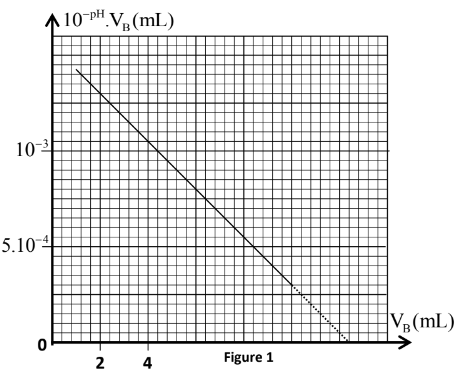
\includegraphics[width=0.5\textwidth]{./img/new_vache.png}
  \end{center}
\end{wrapfigure}



  Un technicien de laboratoire dose l’acidité d’un lait de vache. Il réalise le titrage pH-métrique à l’aide de la
  solution aqueuse $(S_B)$ d’hydroxyde de sodium de concentration molaire $C_B$. Pour cela il introduit , dans un
bécher un volume $V_A = 25,0mL$
de lait, puis il verse progressivement un volume $V_B$
de la solution $(S_B)$ et note
pour chaque volume versé le pH du mélange réactionnel.

On note $V_{BE}$
le volume de la solution d’hydroxyde de sodium versé à l’équivalence et
  $K_A$ la constante d’acidité du couple $HA_{(aq)}/ A^-_{(aq)}$.

  \begin{enumerate}
    \item[2-1] Ecrire l’équation chimique modélisant la réaction du dosage. (0,5pt)
    \item[2-2] Etablir la relation permettant de déterminer la concentration $C_A$ en acide lactique du lait en fonction de $V_A, C_B$ et $V_BE$.(0,5pt)
    \item[2-3] Etablir la relation : $V_B.10^{-pH} = K_A.(V_{BE} - V_B)$ avec $0<V_B<V_{BE}$.(0,75pt)
    \item[2-4] La courbe de la figure 1 représente les variations de $10^{-pH}$ en fonction de $V_B$ : $10^{-pH}.V_B$=$ f(V_B)$.En s’aidant de la courbe de la figure 1.
      \begin{enumerate}
        \item[2-4-1] Déterminer le volume $V_{BE}$ et en déduire la concentration $C_A$.(0.5pt)
        \item[2-4-2] déterminer le $pK_A$ du couple $HA_{(aq)}/ A^-_{(aq)}$ (0.5pt)
      \end{enumerate}
  \end{enumerate}


\end{Box2}
\begin{center}
 \hrulefill
  \Large{--Mécanique--}
\hrulefill\\

\end{center}
%\vspace{-1.0cm}

 \begin{Box2}{SN2023:Mouvement d’un projectile dans le champ de pesanteur uniforme}


  \begin{wrapfigure}[7]{r}{0.24\textwidth}
  \begin{center}
%	  \vspace{-2cm}
	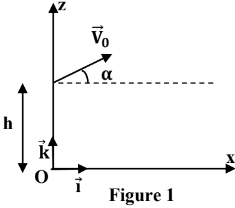
\includegraphics[width=0.25\textwidth]{./img/chute_libre.png}
  \end{center}
\end{wrapfigure}


   \emph{Le but de cette partie est de déterminer la valeur de l’intensité du champ de pesanteur
   $g$ à une faible altitude}
   
   A un instant de date
t=0 , on lance d’un point situé à une hauteur h de la surface de la Terre, un projectile de
masse $m$, avec une vitesse initiale dont le vecteur $\vec{V_0}$ fait un angle $\alpha$
avec l’axe horizontal $(O,\vec{i})$ .

On néglige l’action de l’air et on étudie le mouvement du centre
d’inertie G du projectile dans le repère d’espace $(O, \vec{i}, \vec{k})$
lié à un référentiel terrestre supposé galiléen (figure 1).

La position de $G$ est repérée, à un instant t, par ses coordonnées (x,z) .

\begin{enumerate}
  \item Trouver, en appliquant la deuxième loi de Newton, les expressions
    des composantes $v_x(t)$ et $v_z(t)$ du vecteur vitesse de G.\textbf(0,25pt)
  \item Exprimer la norme $v$ du vecteur vitesse en fonction de $g, \alpha, v_0$ et $t$. \textbf(0,25pt)
  \item 3- La courbe de la figure 2 représente les variations de $v$ en fonction du temps. En exploitant la courbe, trouver :
    \begin{enumerate}
      \item La valeur $V_0$ de la vitesse initiale. (0,25pt)
      \item Les valeurs des composantes $V_{0x}$ et $V_{0z}$ du vecteur vitesse (0,25pt)
    \end{enumerate}
  \item Vérifier que: $\alpha \simeq 30^{\circ}$
  \item La courbe de la figure 3 représente la trajectoire du
mouvement de G dans le repère $(o, \vec{i}, \vec{j})$.
    Soient $\Delta{t_1}$ la durée de passage du projectile de la position
$M_1$ à la position $N_1$ situées à la même altitude
$z_1$ et $\Delta{t_2}$ la
durée de passage du projectile de la position $M_2$ à la position $N_2$ situées à la même altitude telles que $z_2 > z_1$(Figure 3).
\begin{enumerate}
  \item En se basant sur l’équation horaire $z =f(t)$ , vérifier que $$\Delta{t_1} = t_{N_1} - t_{M_1} = \frac{2.\sqrt{(V_0sin\alpha)^2 + 2g(h-z_1)}}{g}$$ avec $t_{M_1}$ l’instant de passage de
G par la position $M_1$ et $t_{N_1}$ l’instant de son passage par $N_1$.(0,5pt)
\item Soit $H= z_2 - z_1$, établir l’expression: $H = \frac{g}{8}((\Delta{t_1})^2 - (\Delta{t_2})^2 )$ et déduire la valeur de g sachant que $\Delta{t_1} = 0,7s$, $\Delta{t_2} = 0,3s$ et H=0,49m.(0,5pt)
\end{enumerate}
\end{enumerate}
  \begin{center}
%	  \vspace{-2cm}
	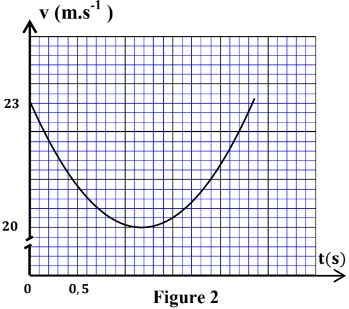
\includegraphics[width=0.46\textwidth]{./img/vitesse_courbe.png}
	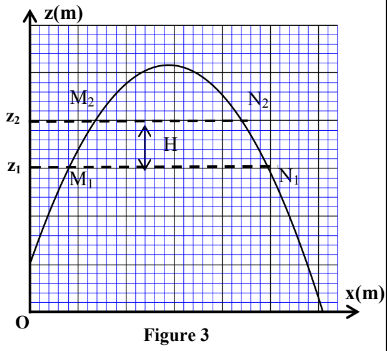
\includegraphics[width=0.46\textwidth]{./img/pos_courbe.png}
  \end{center}
 \end{Box2}


\begin{Box2}{SN2020:Mouvement d’un jouet sur une gouttière}
  \emph{Un jouet modélisé par un solide (S) de masse m = 50g et de centre d’inertie G est abandonné sans vitesse
initiale en un point A d’une gouttière ABCD(figure1). Cette gouttière est constituée:}

\begin{itemize}
  \item d’un tronçon rectiligne AB incliné d’un angle $\alpha =30^{\circ}$ par rapport au plan horizontal et de longueur
$AB = 1,6 m$.
\item d’un tronçon horizontal $BC$.
\item d’un tronçon circulaire $CD$ de centre $O$ et de rayon $r$ et tel que $OC$ est perpendiculaire à $BC$.
\item Intensité de la pesanteur $g =10m.s^{-2}$ .
\end{itemize}

  \begin{center}
%	  \vspace{-2cm}
	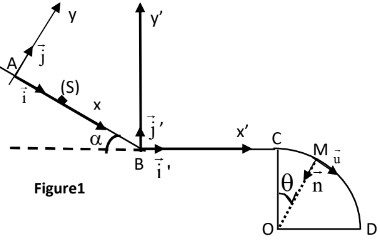
\includegraphics[width=0.46\textwidth]{./img/loi_exo.png}
  \end{center}

La trajectoire du mouvement de (S) se trouve dans un plan vertical.

  On étudie le mouvement du solide (S) sur le parcours AB dans un repère orthonormé $R(A,\vec{i}, \vec{j})$, et son

  mouvement sur le parcours BC dans un repère orthonormé $R(B,\vec{i'}, \vec{j'})$
. Les deux repères sont liés à un
référentiel terrestre supposé galiléen.
  \textbf{Tronçon AB :}
  Le long du parcours AB les frottements sont
négligeables.

\begin{enumerate}
  \item[1-1] Calculer la durée AB t du parcours AB.(0,5pt) 
  \item[1-2]1-2-Déduire que la valeur de la vitesse de (S) à son
arrivée au point B est $V_B = 4 m/s$(0,25pt)
\end{enumerate}

  \textbf{2-Tronçon BC :}
Le long du parcours BC la force de frottement $\vec{f}$
qui s’applique sur (S) est horizontale , de sens contraire à la vitesse de (S) et d’intensité constante.
On considère que le changement de direction au point B n’a pas d’influence sur la valeur de la vitesse.
  Trouver l’intensité f sachant que la durée du parcours $BC$ est $t_{BC} = 0,5s$ et que (S) arrive en C avec une
vitesse nulle.(0,5pt)

  \textbf{3-Tronçon CD :}
Le long du parcours CD les frottements sont négligeables. Le solide (S) part du point C avec une vitesse pratiquement
nulle et aborde le tronçon circulaire CD. La position de G en un point M de CD est repérée par l’angle $\theta = (\vec{OC}, \vec{OM})$

\begin{enumerate}
  \item[3-1] En se basant sur l’application de la deuxième loi de Newton sur (S) dans la base de Freinet $(M, \vec{u}, \vec{n})$(figure 1) :
    \begin{enumerate}
      \item[3-1-1] Trouver l’expression de R l’intensité de la réaction de la gouttière sur (S) au point M en fonction de $m,\theta, r$ et $\dot{\theta} = \frac{d\theta}{dt}$ vitesse angulaire du mouvement de (S).(0,25pt)
      \item[3-1-2] Exprimer l’accélération angulaire $\ddot{\theta}$ en fonction de g, $\theta$ et r.(0,25pt)
    \end{enumerate}
  \item[3-2] 3-2- A partir de l’expression de $\ddot{\theta}$ on a : $\dot{\theta} = \sqrt{\frac{2.g}{r}.(1-cos\theta)}$.En déduire l’expression de R en fonction de
m,g et $\theta$. (0,25pt)
\item[3-3] Pour quelle valeur de $\theta$ le solide (S) quitte la gouttière ? (0,25pt)
\end{enumerate}
\end{Box2}



\end{document}
